\documentclass{article}
\usepackage{graphicx}

\title{Intrusion Detection System (IDS) Report}
\author{Hagay Cohen, Imri Shai}
\date{\today}

\begin{document}

\maketitle

\section{Conclusions from the R\&D}
The research we conducted on data leak attacks provided valuable insights into the types of attacks, methods of exfiltration, and detection mechanisms. We found that data leak attacks can be detected through packet inspection, user behavior analytics, and packet header analysis. These detection methods are implemented in our Intrusion Detection System (IDS) as discribed below.


\section{System Architecture}
Our IDS is designed to monitor network traffic and detect suspicious activities that may indicate data leaks. 
The system architecture is shown in Figure \ref{fig:architecture}.
The IDS consists of three main components: flow classifier, detection engine, and statistical analysis module.
\begin{figure}[h!]
    \centering
    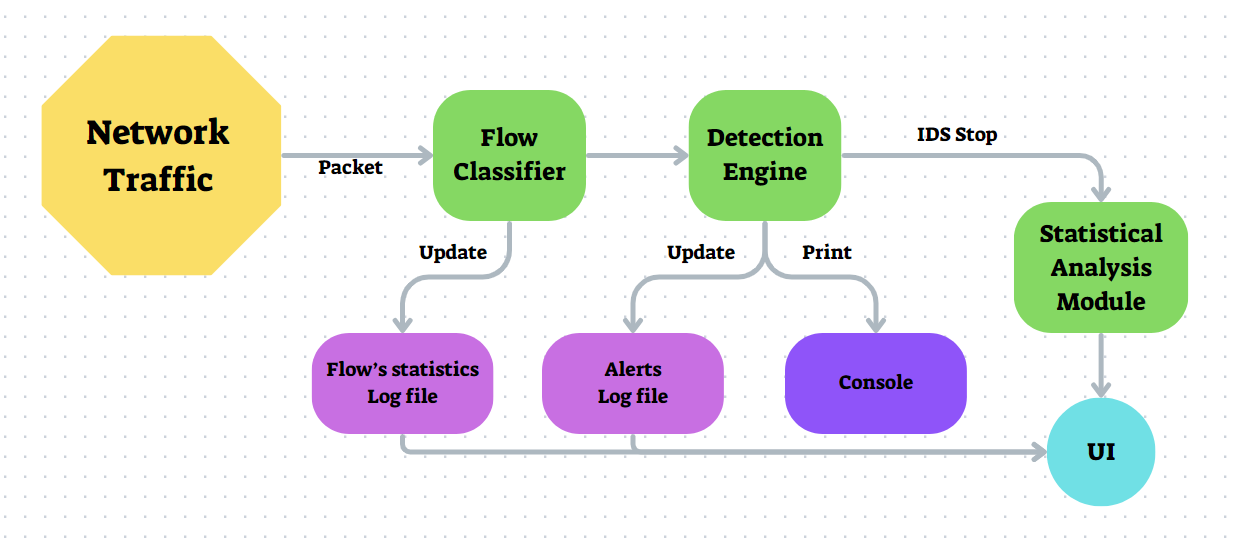
\includegraphics[width=\textwidth]{Screenshots/fig_1.png}
    \caption{System Architecture}
    \label{fig:architecture}
\end{figure}

\subsection{Flow Classifier}
For each packet, the flow classifier extracts a 5-tuple key (source IP, destination IP, source port, destination port, protocol) and assigns it to a flow.
The flow classifier then updates the flow's statistics, such as packet count and byte count, and forwards the flow to the detection engine.

\subsection{Detection Engine}
The detection engine analyzes the flows received from the flow classifier to identify potential data leak attacks.
It uses a set of rules and traffic patterns to detect suspicious activities, such as tunneling, social engineering, and backdoors misuse.
When a potential attack is detected, the detection engine generates an alert, prints it to the console, saves it to a log file.

\subsection{Statistical Analysis Module}
When the IDS is ordered to stop, by gracefully shutting down or an end of a simulation, the statistical analysis module saves the statistics of the flows to a file.
And then, it activates the UI module to display the statistics in a user-friendly way.
All the alerts, flow data, and statistics imgaes are saved to further analysis.
UI example is shown in Appendix \ref{sec:ui}.

\section{Detections Explanations}
Our IDS is capable of detecting various types of intrusions. The detection mechanisms include:
\begin{itemize}
    \item \textbf{Data Exfiltration:} Detects data leak attacks by analyzing packet headers and inspecting packet contents, while considering protocol-specific characteristics.
    \item \textbf{Backdoors Misuse:} Detects backdoors misuse by monitoring network traffic and identifying usege of known backdoor ports or usege of internal protocols.
    \item \textbf{Tunneling:} Identifies tunneling attacks by analyzing packet headers and detecting anomalies in network traffic.
    \item \textbf{Suspicious User Behavior:} Analyzes user behavior and identifies patterns that deviate from normal activities, such as excessive data transfer or after-hours access.
    \item \textbf{Unauthorized IP Address:} Detects unauthorized IP addresses by monitoring network traffic and identifying connections from unknown or blacklisted IP addresses.
\end{itemize}

% add subsections for each detection mechanism

\section{Docker Network Simulation}
We used Docker to simulate a network environment for testing our IDS. The setup includes containers for an internal server, a database, user machines, an external server, and the IDS itself.

\subsection{Network Setup}
The network is defined using a Docker Compose file with the following components:
\begin{itemize}
    \item \textbf{Internal Server:} Nginx web server.
    \item \textbf{Database:} MySQL database.
    \item \textbf{User Machines:} Simulate normal and malicious activities.
    \item \textbf{External Server:} Simulates external threats.
    \item \textbf{IDS:} Monitors and detects suspicious activities.
\end{itemize}

\subsection{Traffic Generation}
Scripts in user containers generate normal and malicious traffic, including web browsing, and data exfiltration.

\subsection{IDS Monitoring and Detection}
The IDS inspects packets, analyzes user behavior, and examines packet headers to detect data leaks. Alerts and logs are generated for suspicious activities.

\subsection{Results and Analysis}
The IDS's effectiveness is evaluated by reviewing alerts and analyzing traffic patterns to identify vulnerabilities.
\section{Test Cases}
In the "volumes" directory under the "ids\_scripts" folder, there is a file named \texttt{Test.py} that contains the test cases. The test cases are designed to validate the functionality of the IDS by simulating various attack scenarios and verifying that the IDS correctly identifies and generates alerts for these attacks. The test cases include:

\begin{itemize}
    \item DNS Tunneling
    \item ICMP Tunneling
    \item Unauthorized Port Access
    \item After Business Hours Traffic
    \item Large Data Transfer
    \item Suspicious Traffic
    \item Unauthorized File Transfer
    \item Unusual Traffic
    \item Unusual User Activity
\end{itemize}

The test cases are executed by running the \texttt{Test.py} script, which generates traffic in PCAP format. The PCAP files can be analyzed using Wireshark and used as input to the IDS for detection.

\section{Future Extensions}
In the future, the IDS can be extended to include more sophisticated detection mechanisms, such as:
\begin{itemize}
    \item \textbf{Machine Learning:} Implement machine learning algorithms to improve detection accuracy and reduce false positives.
    \item \textbf{Deep Packet Inspection:} Analyze packet contents to detect data leaks and identify malicious payloads.
    \item \textbf{Behavioral Analysis:} Monitor user behavior and identify patterns that deviate from normal activities.
    \item \textbf{Sandboxing:} Isolate suspicious files or applications in a sandbox environment to prevent data leaks.
\end{itemize}
\section{Conclusions and Notes}
The IDS is a powerful tool for detecting data leak attacks, backdoors misuse, tunneling, and other security threats. After conducting research on data leak attacks and implementing the IDS, we have gained valuable insights into intrusion detection mechanisms and network security. The IDS can be further enhanced and diversified to address emerging threats and vulnerabilities in network environments.

\textbf{NOTE:} The IDS is a proof-of-concept implementation. In a real-world scenario, the IDS would be deployed in a production environment with additional security measures and monitoring capabilities. Moreover, our IDS is designed to inspect unencrypted network traffic. Encrypted traffic, which is a common practice in modern networks, would require additional mechanisms, and some of the detection mechanisms may not be applicable.

\appendix

\section{User Interface Example}
\label{sec:ui}
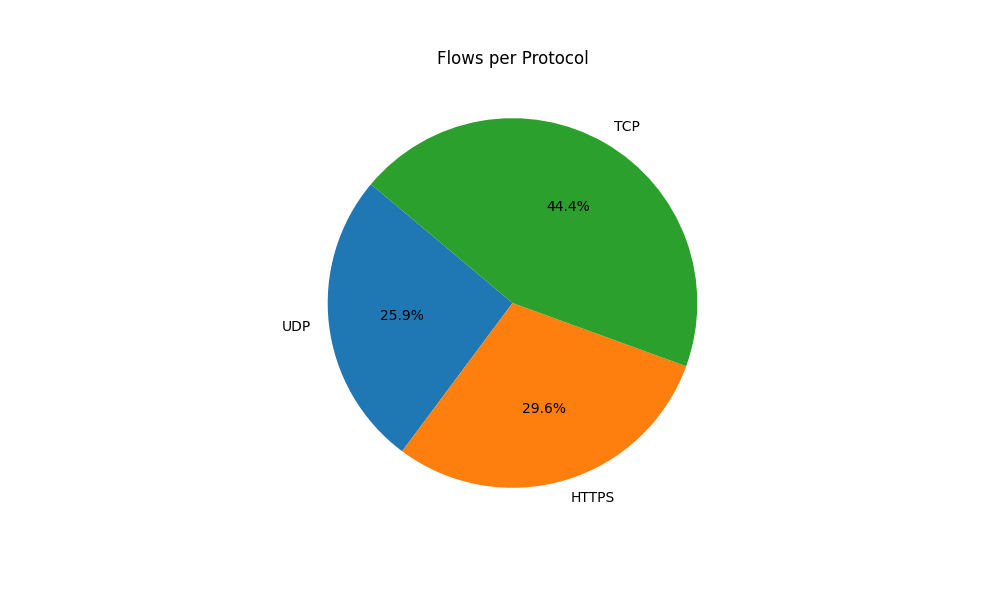
\includegraphics[width=\textwidth]{Screenshots/Flows_per_Protocol.png}
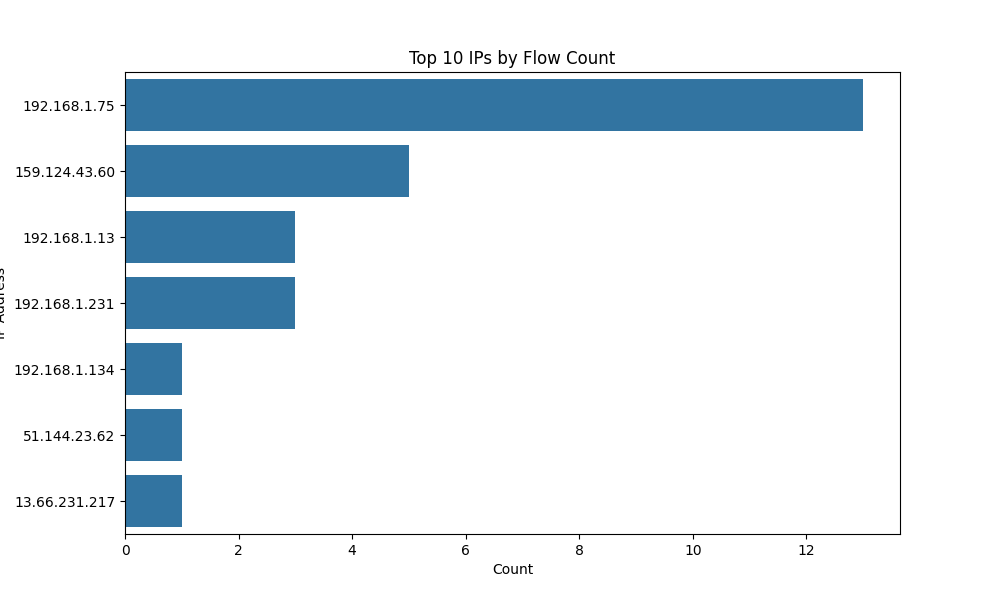
\includegraphics[width=\textwidth]{Screenshots/Top_10_IPs_by_Flow_Count.png}
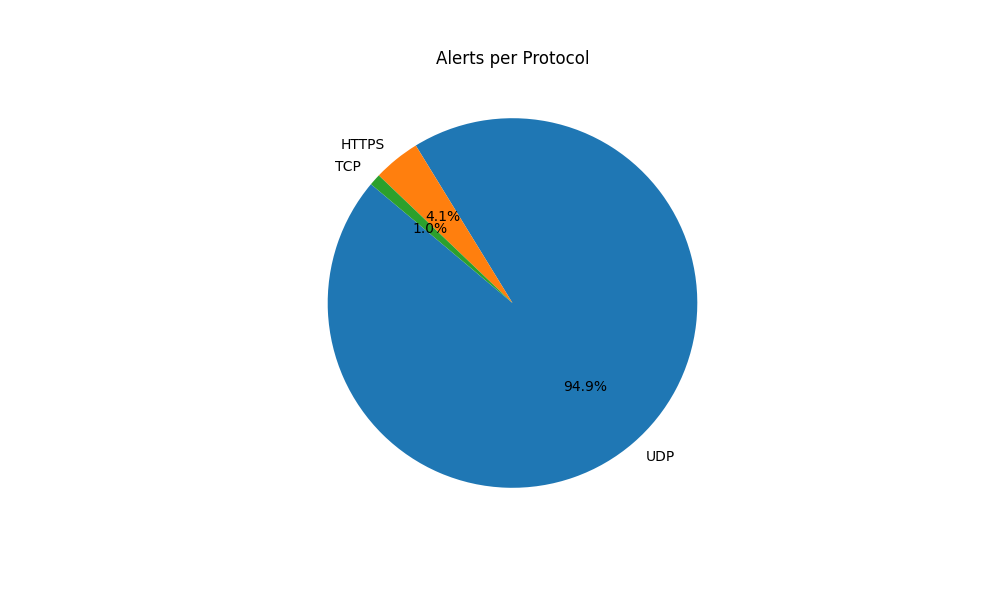
\includegraphics[width=\textwidth]{Screenshots/Alerts_per_Protocol.png}
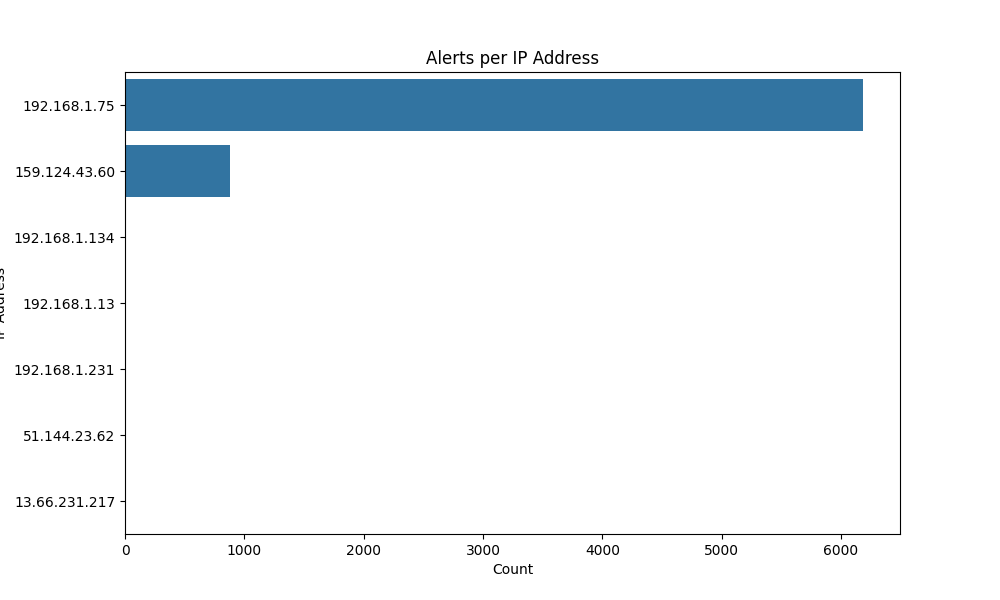
\includegraphics[width=\textwidth]{Screenshots/Alerts_per_IP_Address.png}


\end{document}